%TODO: Reorder, entzerren

\documentclass[%handout,
	sans,
	12pt,
	%slidescentered,% center text on slide
	%draft,			% compile as draft version
	%notes,			% include nodes in slides
	%compress		% compress navigation bar
]{beamer}

\beamertemplatenavigationsymbolsempty

\setbeamertemplate{frametitle}
{
    \vspace*{1.5em}\insertframetitle\vspace*{-1.5em}
}


\usepackage[T1]{fontenc}
\usepackage[utf8x]{inputenc}

\usepackage{mathpazo}
\usepackage[british]{babel}
\usepackage{csquotes}

\usepackage{svg}

\newcommand{\high}[1]{{\usebeamercolor[fg]{structure} #1}}
\newcommand{\bad}[1]{\textcolor{red}{#1}}
\newcommand{\gray}[1]{\textcolor{darkgray}{#1}}
\newcommand{\black}[1]{\textcolor{black}{#1}}

\usepackage{amsmath,amssymb}
\usepackage{upgreek}
\usepackage{booktabs}
\usepackage{hyperref}
\usepackage{default}
\usepackage{graphicx}
\usepackage{colortbl}
\usepackage{url}
\usepackage{setspace}
\usepackage{wrapfig}
\usepackage{tabularx}
\usepackage{pgfplots}
\pgfplotsset{compat=1.9}
\usepackage{tikz}
\usepackage{pgfplotstable}

\usetikzlibrary{snakes,arrows,shapes}

\setbeamertemplate{caption}[numbered]

\newcommand{\RR}{\mathbb{R}}
\newcommand{\NN}{\mathbb{N}}
\def\braces#1{[#1]}

%\definecolor{mybg}{rgb}{0.9,0.9,0.9}
\definecolor{mybg}{rgb}{1,1,1}
\setbeamercolor{background canvas}{bg=mybg}

\title{An executables specification of BDDs in Isabelle}
\author{\normalsize Max Haslbeck and Julius Michaelis}
\institute[]{\footnotesize Fakultät für Informatik\\TU München}
\date{\footnotesize 26 February 2016}

\begin{document}

\maketitle


\section{Introduction - BDDs}
\begin{frame}{Introduction - BDDs}
\begin{center}
\begin{figure}
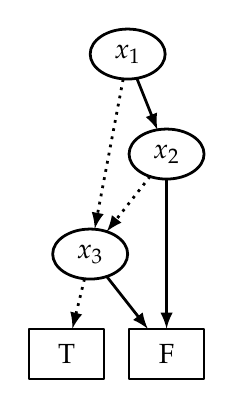
\begin{tikzpicture}[>=latex,line join=bevel,scale=0.5]
  \pgfsetlinewidth{1bp}
%%
\pgfsetcolor{black}
  % Edge: 10 -> 9
  \draw [->] (77.636bp,216.41bp) .. controls (80.913bp,208.22bp) and (84.944bp,198.14bp)  .. (92.412bp,179.47bp);
  % Edge: 9 -> 3
  \draw [->,dotted] (87.066bp,145.81bp) .. controls (79.786bp,136.55bp) and (70.337bp,124.52bp)  .. (55.911bp,106.16bp);
  % Edge: 9 -> 0
  \draw [->] (99bp,143.87bp) .. controls (99bp,119.67bp) and (99bp,75.211bp)  .. (99bp,36.189bp);
  % Edge: 3 -> 0
  \draw [->] (55.934bp,73.811bp) .. controls (62.747bp,65.141bp) and (71.459bp,54.052bp)  .. (85.543bp,36.127bp);
  % Edge: 10 -> 3
  \draw [->,dotted] (67.743bp,215.87bp) .. controls (63.142bp,191.67bp) and (54.688bp,147.21bp)  .. (47.268bp,108.19bp);
  % Edge: 3 -> 1
  \draw [->,dotted] (39.885bp,72.055bp) .. controls (37.992bp,64.261bp) and (35.7bp,54.822bp)  .. (31.195bp,36.275bp);
  % Node: 9
\begin{scope}
  \definecolor{strokecol}{rgb}{0.0,0.0,0.0};
  \pgfsetstrokecolor{strokecol}
  \draw (99bp,162bp) ellipse (27bp and 18bp);
  \draw (99bp,162bp) node {$x_2$};
\end{scope}
  % Node: 10
\begin{scope}
  \definecolor{strokecol}{rgb}{0.0,0.0,0.0};
  \pgfsetstrokecolor{strokecol}
  \draw (71bp,234bp) ellipse (27bp and 18bp);
  \draw (71bp,234bp) node {$x_1$};
\end{scope}
  % Node: 3
\begin{scope}
  \definecolor{strokecol}{rgb}{0.0,0.0,0.0};
  \pgfsetstrokecolor{strokecol}
  \draw (44bp,90bp) ellipse (27bp and 18bp);
  \draw (44bp,90bp) node {$x_3$};
\end{scope}
  % Node: 1
\begin{scope}
  \definecolor{strokecol}{rgb}{0.0,0.0,0.0};
  \pgfsetstrokecolor{strokecol}
  \draw (54bp,36bp) -- (0bp,36bp) -- (0bp,0bp) -- (54bp,0bp) -- cycle;
  \draw (27bp,18bp) node {T};
\end{scope}
  % Node: 0
\begin{scope}
  \definecolor{strokecol}{rgb}{0.0,0.0,0.0};
  \pgfsetstrokecolor{strokecol}
  \draw (126bp,36bp) -- (72bp,36bp) -- (72bp,0bp) -- (126bp,0bp) -- cycle;
  \draw (99bp,18bp) node {F};
\end{scope}
%
\end{tikzpicture}
\caption{$(\overline{x_1} \land \overline{x_3}) \lor (\overline{x_2} \land 
          \overline{x_3})$}
\end{figure}

  \textbf{BDD} = Binary Decision Diagram \\
  \textbf{ROBDD} = Reduced Ordered Binary Decision Diagram
\end{center}
\end{frame}


\begin{frame}{Boolean functions}
\begingroup
\addtolength{\jot}{-1mm}
{\footnotesize
\begin{flalign*}
  \onslide<1->{
    &\textbf{type\_synonym}\ \tau\ bf\ \textbf{=}\ (\tau \Rightarrow bool)
    \Rightarrow bool &
    }
  \onslide<2->{
  \\[1\baselineskip]
    & \textbf{definition}\ \textit{bf-ite}\ ::\ \tau\ bf \Rightarrow
    \tau\ bf \Rightarrow \tau\ bf \Rightarrow \tau\ bf\ \textbf{where} &
  \\
    &\hskip4mm   \textit{bf-ite}\ i\ t\ e\ =\ (\lambda x.\ \text{if}\ i\ x\
    \text{then}\ t\ x\ \text{else}\ e\ x)&
  }
  \onslide<3->{
  \\[1\baselineskip]
    &\textbf{definition}\ \textit{bf-restrict}\ ::\ \tau\ bf \Rightarrow \tau
    \Rightarrow bool \Rightarrow \tau\ bf\ \textbf{where}&
  \\
    &\hskip4mm \textit{bf-restrict}\ f\ v\ b\ =\ (\lambda a.\ f\ (a(v := b))&
  }
  \onslide<4->{
  \\[1\baselineskip]
    & \textbf{lemma:}\ \textit{bf-ite}\ I\ T\ E\ =&
  \\
    &\phantom{\textbf{lemma:}}\ \textit{bf-ite}\ (\lambda l.\ l\ v)&
  \\
    &\phantom{\textbf{lemma:}\ \textit{bf-ite}}\
    (\textit{bf-ite}\ (\textit{bf-restrict}\ I\ v\ \textit{True})\
    (\textit{bf-restrict}\ T\ v\ \textit{True})&
  \\
    &\phantom{\textbf{lemma:}\ \textit{bf-ite}\ (\textit{bf-ite}}\
    (\textit{bf-restrict}\ E\ v\ \textit{True}))&
  \\
    &\phantom{\textbf{lemma:}\ \textit{bf-ite}}\
    (\textit{bf-ite}\ (\textit{bf-restrict}\ I\ v\ \textit{False})\
    (\textit{bf-restrict}\ T\ v\ \textit{False})&
  \\
    &\phantom{\textbf{lemma:}\ \textit{bf-ite}\ (\textit{bf-ite}}\
    (\textit{bf-restrict}\ E\ v\ \textit{False}))&
  }
\end{flalign*}
}
\endgroup
\vspace*{-10mm}
\end{frame}


\begin{frame}<1-2>[label=bdtformulas]{Binary Decision Trees}
\begingroup
\addtolength{\jot}{-1mm}
{\footnotesize
\begin{flalign*}
   \visible<1->{
   &\textbf{datatype}\ (\tau :: \textit{linorder})\ \textit{bdt}\ \textbf{=}\
    \textit{Trueif}\ |\ \textit{Falseif}\ |\ IF\ \tau\ (\tau\ \textit{bdt})\
    (\tau\ \textit{bdt}) &
  }
  \visible<2->{
  \\[\baselineskip]
  &\textbf{definition}\
    \textit{bf-bdt-rel}\ = \{(bf, bd).\ \textit{ro-bdt}\ bd\ \land\ \forall a.\
    bf\ a = \textit{val-bdt}\ bd\ a\} &
  }
  \visible<3->{
  \\[\baselineskip]
    & \textbf{lemma:}\
    (bf,bd) \in \textit{bf-bdt-rel} \Longrightarrow (bf',bd') \in
    \textit{bf-bdt-rel}& \\ & \phantom{lemma:}\ \Longrightarrow  (bf = bf')
    \leftrightarrow (bd = bd') &
  }
  \visible<4->{
  \\[\baselineskip]
    &\textbf{lemma:}\ (i,ibd) \in
    \textit{bf-bdt-rel} \Longrightarrow (t,tbd) \in \textit{bf-bdt-rel}&
  \\
    &\phantom{lemma:}\Longrightarrow (e,ebd) \in \textit{bf-bdt-rel} & \\ &
    \phantom{lemma:}\Longrightarrow (\textit{bf-ite}\ i\ t\ e, \textit{bdt-ite}\
    ibd\ tbd\ ebd) \in \textit{bf-bdt-rel}&
  }
\end{flalign*}
}
\endgroup
\vspace*{-10mm}
\end{frame}


\begin{frame}[label=bdtgraph]{Binary Decision Trees}
\begin{center}
\begin{figure}
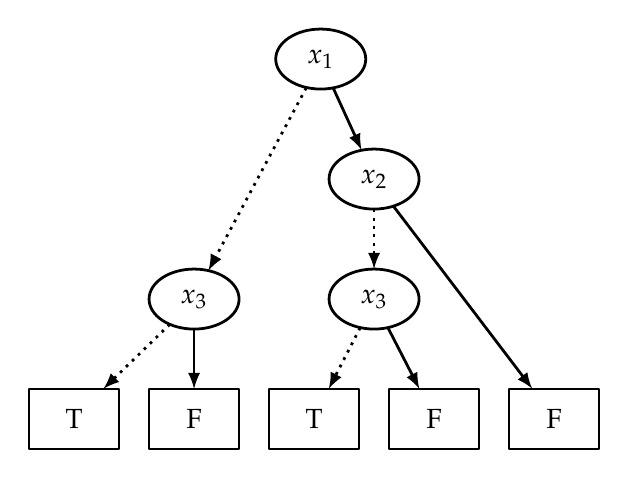
\begin{tikzpicture}[>=latex,line join=bevel,scale=0.6]
  \pgfsetlinewidth{1bp}
%%
\begin{scope}
  \pgfsetstrokecolor{black}
  \definecolor{strokecol}{rgb}{1.0,1.0,1.0};
  \pgfsetstrokecolor{strokecol}
  \definecolor{fillcol}{rgb}{1.0,1.0,1.0};
  \pgfsetfillcolor{fillcol}
  \filldraw (0bp,0bp) -- (0bp,252bp) -- (342bp,252bp) -- (342bp,0bp) -- cycle;
\end{scope}
\begin{scope}
  \pgfsetstrokecolor{black}
  \definecolor{strokecol}{rgb}{1.0,1.0,1.0};
  \pgfsetstrokecolor{strokecol}
  \definecolor{fillcol}{rgb}{1.0,1.0,1.0};
  \pgfsetfillcolor{fillcol}
  \filldraw (0bp,0bp) -- (0bp,252bp) -- (342bp,252bp) -- (342bp,0bp) -- cycle;
\end{scope}
  \pgfsetcolor{black}
  % Edge: x32 -> 10
  \draw [->] (215.35bp,72.765bp) .. controls (219.54bp,64.611bp) and (224.73bp,54.529bp)  .. (234.19bp,36.124bp);
  % Edge: x32 -> 11
  \draw [->,dotted] (198.65bp,72.765bp) .. controls (194.46bp,64.611bp) and (189.27bp,54.529bp)  .. (179.81bp,36.124bp);
  % Edge: x1 -> x2
  \draw [->] (182.58bp,216.41bp) .. controls (186.37bp,208.13bp) and (191.03bp,197.92bp)  .. (199.47bp,179.47bp);
  % Edge: x2 -> 30
  \draw [->] (218.76bp,145.53bp) .. controls (237.27bp,121.2bp) and (273.39bp,73.714bp)  .. (301.91bp,36.21bp);
  % Edge: x2 -> x32
  \draw [->,dotted] (207bp,143.7bp) .. controls (207bp,135.98bp) and (207bp,126.71bp)  .. (207bp,108.1bp);
  % Edge: x31 -> 20
  \draw [->] (99bp,71.697bp) .. controls (99bp,63.983bp) and (99bp,54.712bp)  .. (99bp,36.104bp);
  % Edge: x1 -> x31
  \draw [->,dotted] (166.28bp,216.71bp) .. controls (153.11bp,192.1bp) and (128.03bp,145.24bp)  .. (107.62bp,107.1bp);
  % Edge: x31 -> 21
  \draw [->,dotted] (84.43bp,74.834bp) .. controls (75.082bp,65.746bp) and (62.702bp,53.71bp)  .. (44.602bp,36.113bp);
  % Node: x32
\begin{scope}
  \definecolor{strokecol}{rgb}{0.0,0.0,0.0};
  \pgfsetstrokecolor{strokecol}
  \draw (207bp,90bp) ellipse (27bp and 18bp);
  \draw (207bp,90bp) node {$x_3$};
\end{scope}
  % Node: 11
\begin{scope}
  \definecolor{strokecol}{rgb}{0.0,0.0,0.0};
  \pgfsetstrokecolor{strokecol}
  \draw (198bp,36bp) -- (144bp,36bp) -- (144bp,0bp) -- (198bp,0bp) -- cycle;
  \draw (171bp,18bp) node {T};
\end{scope}
  % Node: x31
\begin{scope}
  \definecolor{strokecol}{rgb}{0.0,0.0,0.0};
  \pgfsetstrokecolor{strokecol}
  \draw (99bp,90bp) ellipse (27bp and 18bp);
  \draw (99bp,90bp) node {$x_3$};
\end{scope}
  % Node: 20
\begin{scope}
  \definecolor{strokecol}{rgb}{0.0,0.0,0.0};
  \pgfsetstrokecolor{strokecol}
  \draw (126bp,36bp) -- (72bp,36bp) -- (72bp,0bp) -- (126bp,0bp) -- cycle;
  \draw (99bp,18bp) node {F};
\end{scope}
  % Node: 21
\begin{scope}
  \definecolor{strokecol}{rgb}{0.0,0.0,0.0};
  \pgfsetstrokecolor{strokecol}
  \draw (54bp,36bp) -- (0bp,36bp) -- (0bp,0bp) -- (54bp,0bp) -- cycle;
  \draw (27bp,18bp) node {T};
\end{scope}
  % Node: 10
\begin{scope}
  \definecolor{strokecol}{rgb}{0.0,0.0,0.0};
  \pgfsetstrokecolor{strokecol}
  \draw (270bp,36bp) -- (216bp,36bp) -- (216bp,0bp) -- (270bp,0bp) -- cycle;
  \draw (243bp,18bp) node {F};
\end{scope}
  % Node: 30
\begin{scope}
  \definecolor{strokecol}{rgb}{0.0,0.0,0.0};
  \pgfsetstrokecolor{strokecol}
  \draw (342bp,36bp) -- (288bp,36bp) -- (288bp,0bp) -- (342bp,0bp) -- cycle;
  \draw (315bp,18bp) node {F};
\end{scope}
  % Node: x2
\begin{scope}
  \definecolor{strokecol}{rgb}{0.0,0.0,0.0};
  \pgfsetstrokecolor{strokecol}
  \draw (207bp,162bp) ellipse (27bp and 18bp);
  \draw (207bp,162bp) node {$x_2$};
\end{scope}
  % Node: x1
\begin{scope}
  \definecolor{strokecol}{rgb}{0.0,0.0,0.0};
  \pgfsetstrokecolor{strokecol}
  \draw (175bp,234bp) ellipse (27bp and 18bp);
  \draw (175bp,234bp) node {$x_1$};
\end{scope}
%
\end{tikzpicture}
\caption{BDT $(\overline{x_1} \land \overline{x_3}) \lor (\overline{x_2} \land 
              \overline{x_3})$}
\end{figure}
\end{center}
\end{frame}


\againframe<3-4>{bdtformulas}


\againframe{bdtgraph}

\begin{frame}{BDDs on abstract datatypes}
\begin{itemize}
  \visible<1->{
  \item usage of Isabelle's locale feature
    \begin{itemize}
      \item define basic operations and respective assumptions
      \item Relation \textit{bdt-bdd-rel}
      }
  \visible<2->{
      \item $ (ib, ibd) \in \textit{bdt-bdd-rel}  \Longrightarrow $ \\
            $(tb, tbd) \in \textit{bdt-bdd-rel} \Longrightarrow $ \\
            $(eb, ebd) \in \textit{bdt-bdd-rel} \Longrightarrow $ \\
            $(\textit{bdt-ite}\ ib\ tb\ eb, \textit{bdd-ite}\ ibd\ tbd\ ebd)
             \in \textit{bdt-bdd-rel} $ \\
      \phantom{Hack for more space between items}
    \end{itemize}
  }
  \visible<3->{
  \item instantiation of locale with abstract datatype \textit{pointermap}
  }
\end{itemize}
\end{frame}


\begin{frame}{Pointermap}
\visible<1->{
\begin{itemize}
  \item given an element, it constructs a pointer (or small representation) to
        that element; it provides equal pointers for equal elements
  \item given a pointer, we can retrieve an element
\end{itemize}
}
\begingroup
\addtolength{\jot}{-1mm}
{\footnotesize
\begin{flalign*}
\visible<2->{
  %TODO: Fugly hack to move to the right
  &\hskip1cm\textbf{record}\ \tau\ \textit{pointermap} =& \\
  %TODO: Im to stupid for correct alignment, whitespace FTW
  &\hskip12mm \textit{entries}\ \ \ ::\ \tau\ \textit{list}& \\
  &\hskip12mm \textit{getentry}\ ::\ \tau\ \Rightarrow \textit{nat}\
  \textit{option}&
}
\visible<3->{
  \\[\baselineskip]
  &\hskip12mm \textbf{fun}\ \textit{pm\_pth} :: \tau\ \textit{pointermap} \Rightarrow 
  \textit{nat} \Rightarrow \tau&
  \\
  &\hskip12mm \textbf{fun}\ \textit{pm\_getmk}\ :: \tau \Rightarrow \tau\ \textit{pointermap}
  \Rightarrow (\textit{nat} \times  \textit{pointermap})&
}
\end{flalign*}
}
\endgroup
\vspace*{-10mm}
\end{frame}


\begin{frame}{Implementation}
\begingroup
{\footnotesize
\begin{flalign*}
  %TODO: Fugly hack to move to the right
  &\hskip1cm\textbf{record}\ \tau\ \textit{pointermap-impl} =&
  \\
  %TODO: Im to stupid for correct alignment, whitespace FTW
  &\hskip12mm \textit{entriesi}\ \ \ ::\ \tau\ \textit{array-list}&
  \\
  &\hskip12mm \textit{getentryi}\ ::\ (\tau, nat)\ \textit{hashtable}&
\end{flalign*}
}
\endgroup

Verification via separation logic:

\begingroup
{\footnotesize
\begin{flalign*}
    &\hskip1cm(ibf, i) \in R \Longrightarrow (tbf, t) \in R \Longrightarrow
    (ebd, e) \in R \Longrightarrow&
  \\
    &\hskip1cm <\textit{bdd-relator}\ R\ S>&
  \\
    &\hskip15mm iteci\ i\ t\ e&
  \\
    &\hskip1cm <\lambda(b,s').\ \textit{bdd-relator}\ 
    (\{(\textit{bf-ite}\ ibf\ tbf\ ebf,b)\} \cup R)\ s'>&
\end{flalign*}
}
\endgroup
\end{frame}


\begin{frame}<1-1>[label=optimization]{Optimization}
  \begin{itemize}
    \visible<1->{
    \item optimize ``naive'' implementation and verify the optimizations step-by-step
    \item first catch obvious cases
         (e.g. $(\textit{bf-ite}\ (\lambda x. \textit{True})\ t\ e)$) in
          \textit{bdd-ite}
    \item add lookup function for memoization of \textit{bdd-ite}:
    }
    \visible<2->{
    \begin{itemize}
      \item using map ($ bdd \times bdd \times bdd \Rightarrow bdd\
            \textit{option} $)
            on abstract level for proving correctness
      \item using hashmap on concrete implementation
    }
    \end{itemize}
\end{itemize}
\end{frame}


\begin{frame}{Memoization example}
    %\item bf-ite F $x_1$ G = bf-ite (x1) (bf-ite F True G) (bf-ite F False G)
    %\item bf-ite F $x_2$ G = bf-ite (x2) (bf-ite F True G) (bf-ite F False G)
\begin{flalign*}
    &\hskip4mm   \textit{bf-ite}\ F\ (\lambda l.\ l\ x_1)\ G\ =\
    \textit{bf-ite}\ (\lambda l.\ l\ x_1)\ 
    \\
    %TODO: to lazy for proper align
    &\hskip47mm(\textit{bf-ite}\ F\ (\lambda l.\ True)\ G)
    \\
    %TODO: to lazy for proper align
    &\hskip47mm(\textit{bf-ite}\ F\ (\lambda l.\ False)\ G)
    \\
    &\hskip4mm   \textit{bf-ite}\ F\ (\lambda l.\ l\ x_2)\ G\ =\
    \textit{bf-ite}\ (\lambda l.\ l\ x_2)\ 
    \\
    %TODO: to lazy for proper align
    &\hskip47mm(\textit{bf-ite}\ F\ (\lambda l.\ True)\ G)
    \\
    %TODO: to lazy for proper align
    &\hskip47mm(\textit{bf-ite}\ F\ (\lambda l.\ False)\ G)
\end{flalign*}
\end{frame}


\againframe<2-2>{optimization}


\begin{frame}{Equivalence/tautology benchmark}
  \begin{center}
	\begin{align*}
	x_1 \longleftrightarrow (x_2 \longleftrightarrow (\dots \longleftrightarrow (x_n \longleftrightarrow \\
	(x_1 \longleftrightarrow (x_2 \longleftrightarrow (\dots \longleftrightarrow x_n))))))
	\end{align*}

	\begin{tikzpicture}[scale=.9]
		\begin{axis}[ylabel=time in s, xlabel=n, ymode=log, legend pos=south east]
      %TODO: fix labels
      \pgfplotsset{every x tick label/.append style={font=\scriptsize}}
			\addplot table [col sep=comma] {csv/urquhart1500.csv};
			\addplot table [col sep=comma] {csv/buddy_urquhart1500.csv};
      \addlegendentry[pos=southwest]{ {\footnotesize Isabelle BDD}}
      \addlegendentry[pos=southwest]{ {\footnotesize Buddy}}
		\end{axis}
	\end{tikzpicture}
  \end{center}
\end{frame}


\begin{frame}{Conclusion}
	\begin{block}{Limitations}
		\begin{itemize}
			\item No garbage collection
			\item No variable reordering
		\end{itemize}
	\end{block}
	\begin{block}{Achievements}
		\begin{itemize}
			\item About a factor of 10 faster than previous work on BDDs in Isabelle
      \item Haskell tool for tautology checking and creating .dot-files
            available
		\end{itemize}
	\end{block}
\end{frame}


\begin{frame}[c]
\begin{center}
Thank you
\end{center}
\end{frame}


\end{document}
